% Title: Subset and equality constraints
% Author: Jakob Voß
%
% This diagram shows how OMR2 symbols for subset and equality constraints
% could be replaces by simple subtyping arrows.
\documentclass{article}
\usepackage{tkz-orm}
\begin{document}
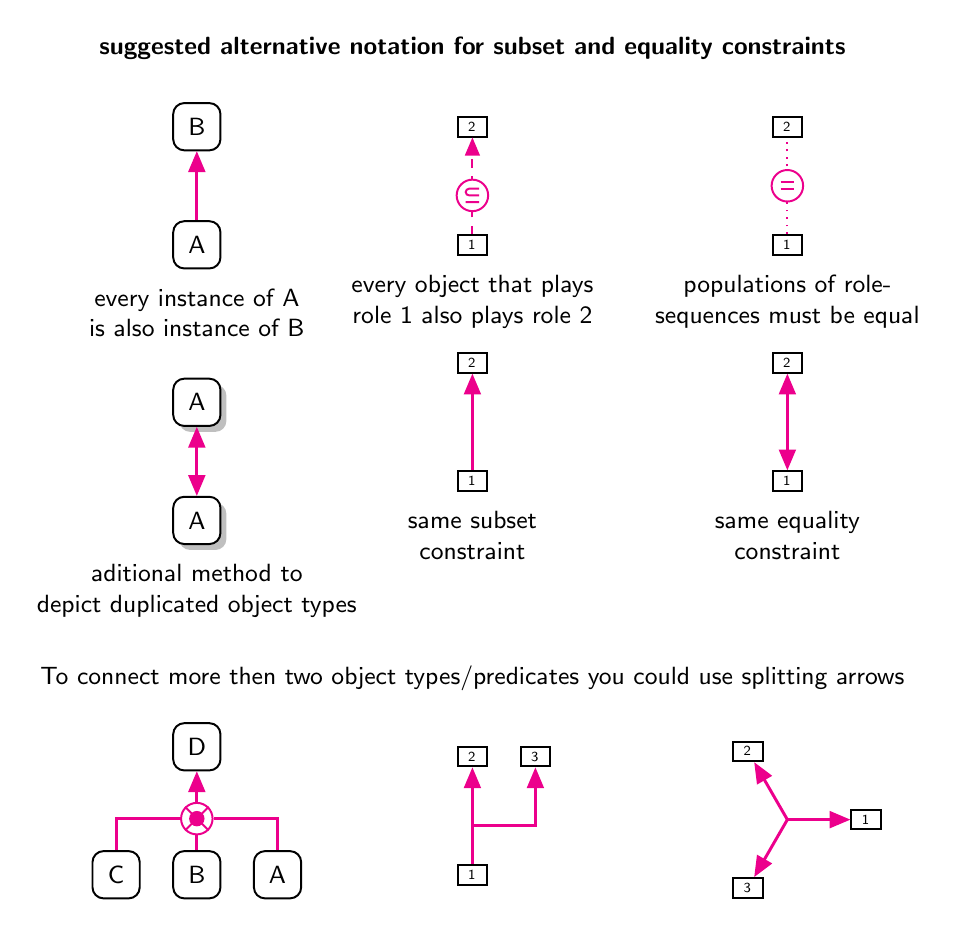
\begin{tikzpicture}[orm]
\node at (3.5,1) {\textbf{suggested alternative notation for
 subset and equality constraints}};
\entity (B) at (0,0) {B};
\entity[label={[align=center]below:every instance of A\\is also instance of B
}] (A) at (0,-1.5) {A};
\draw[subtype] (B) to (A);

\begin{scope}[xshift=3.5cm]
\unary[index=2] (a) at (0,0) {};
\unary[index=1,label={[align=center]below:
every object that plays\\role 1 also plays role 2
}] (b) at (0,-1.5) {};
\limitsto (b) to node[constraint=subset,pos=0.4]{} (a);
\end{scope}

\begin{scope}[yshift=-3.5cm]
\entity[duplicated] (B) at (0,0) {A};
\entity[duplicated,label={[align=center]below:aditional method to\\
depict duplicated object types}] (A) at (0,-1.5) {A};
\draw[subtype,<->] (B) to (A);
\end{scope}

\begin{scope}[xshift=7.5cm]
\unary[index=2] (a) at (0,0) {};
\unary[index=1,label={[align=center]below:
populations of role-\\sequences must be equal
}] (b) at (0,-1.5) {};
\limits (b) to node[constraint=equal]{} (a);
\end{scope}

\begin{scope}[xshift=3.5cm,yshift=-3cm]
\unary[index=2] (a) at (0,0) {};
\unary[index=1,label={[align=center]below:same subset\\constraint}] (b) at (0,-1.5) {};
\draw[subtype] (a) to (b);
\end{scope}

\begin{scope}[xshift=7.5cm,yshift=-3cm]
\unary[index=2] (a) at (0,0) {};
\unary[index=1,label={[align=center]below:same equality\\constraint}] (b) at (0,-1.5) {};
\draw[subtype,<->] (b) to (a);
\end{scope}

\node at (3.5,-7) {To connect more then two object types/predicates you could use splitting arrows};

\begin{scope}[yshift=-9.5cm]
\entity (B) {B};
\entity[right=of B] (A) {A};
\entity[left=of B] (C) {C};
\entity[above=1cm of B] (D) {D};
\draw[subtype] (D) to node[pos=0.6,constraint=xor] (x) {} (B);
\draw[inheritance] (A) |- (x) (C) |- (x);
\end{scope}

\begin{scope}[xshift=3.5cm,yshift=-8cm]
\unary[index=2] (a) at (0,0) {};
\unary[index=3] (b) at (0.8,0) {};
\unary[index=1] (c) at (0,-1.5) {};
\draw[subtype] (a) to coordinate[pos=0.6] (d) (c);
\draw[subtype] (b) |- (d);
\end{scope}

\begin{scope}[xshift=7.5cm,yshift=-8.8cm]
\unary[index=1] at (0:1cm) (a) {};
\unary[index=2] at (120:1cm) (b) {};
\unary[index=3] at (-120:1cm) (c) {};
\draw[suptype] (0,0) to (a);
\draw[suptype] (0,0) to (b);
\draw[suptype] (0,0) to (c);
\end{scope}

\end{tikzpicture}
\end{document}